\documentclass[11pt,a4paper]{article}

\usepackage[utf8]{inputenc}
\usepackage[T1]{fontenc}
\usepackage[ngerman]{babel}
\usepackage{hyperref}
\usepackage{listings}
\usepackage{parskip}
\usepackage{svg}
\usepackage{caption}

\hypersetup{
  colorlinks=true,
  linkcolor=black,
  urlcolor=blue
}

\lstset{
  basicstyle=\ttfamily\small,
  breaklines=true,
  columns=fullflexible
}

\title{Ergebnisbericht: Pi-based Voice Assistant with ESP32-S3}
\date{}

\begin{document}
\maketitle

\section*{1. Einleitung}

Kommerzielle Voice-Assistants wie Siri oder Alexa sind in der Regel nicht Open Source und entsprechend begrenzt auf individuelle Bedürfnisse anpassbar. Vor diesem Hintergrund will ich mit diesem Prototyp einen anderen Ansatz präsentieren: Einen Voice Assistant basierend auf dem Open-Source-Coding-Agenten \href{https://github.com/earendil-works/pi}{Pi}.

Inhaltlich ist das Projekt stark von \href{https://github.com/openclaw/openclaw}{OpenClaw} inspiriert, nur mit Sprache statt Text als Interface. Die Spracheingabe des Voice Assistant läuft über ein Waveshare ESP32-S3 Audio Board, ist aber als beliebig austauschbare Komponente gedacht. Der ESP32 erkennt lokal ein Wakeword, nimmt die Sprache auf, zeigt den Aufnahmezustand über LEDs an und spielt die Antwort wieder ab. Die rechenintensiven Teile laufen nicht über den Mikrocontroller, sondern auf einem separaten Backend innerhalb eines Dockercontainers. Der ESP32 bleibt dadurch bewusst einfach und austauschbar. Die Verwendung von Pi als Agenten-Kern hat den großen Vorteil, dass bestehende Skills und Tools aus bestehenden Agent-Workflows (wie Codex, Claude, OpenClaw, …) leicht integrierbar und wiederverwendbar sind.

Hinweis: Im Root des Repos befindet sich ein Demo-Video des Endergebnisses.

\section*{2. Systemidee}

Die Idee für den Voice-Agenten kommt aus zwei Richtungen: Einerseits von der recht teuren \href{https://developers.openai.com/api/docs/guides/realtime}{OpenAI Realtime API}, welche ich oft zum Lernen von Studieninhalten verwendete, andererseits von dem textbasierten OpenClaw. Ziel war und ist ein Agent, der nicht textbasiert kommuniziert, aber trotzdem günstig, Open Source, erweiterbar und kontrollierbar bleibt. Ich persönlich finde grade für kleine alltägliche Aufgaben Sprache deutlich angenehmer, als textbasierte Kommunikation. Ähnlich wie OpenClaw ist mein Voice Assistant durch seinen Pi-Kern hoch individualisierbar.

Pi wurde ursprünglich vom Österreicher Mario Zechner entwickelt und bildet einen Open-Source-Konkurrenten zu einschlägigen Code-Agenten wie Codex oder Claude. Bekanntheit erlangte Pi durch seine Verwendung in OpenClaw. Pi zeichnet sich durch einen minimalistisch gehaltenen Agentenkern aus, der in TypeScript geschrieben und hoch individualisierbar ist. Pi lässt sich via API-Keys, aber auch über Subscriptions wie ChatGPT Plus nutzen und erlaubt es, System Prompt, Tools, Provider, Profile und Extensions selber anzupassen.
Mittlerweile ist Pi in meinem Coding-Alltag ein fester Bestandteil geworden - sowohl bei meiner Arbeit als auch bei privaten Projekten (wie diesem Prototypen hier).



\section*{3. Architektur}

\begin{figure}[htbp]
    \centering
    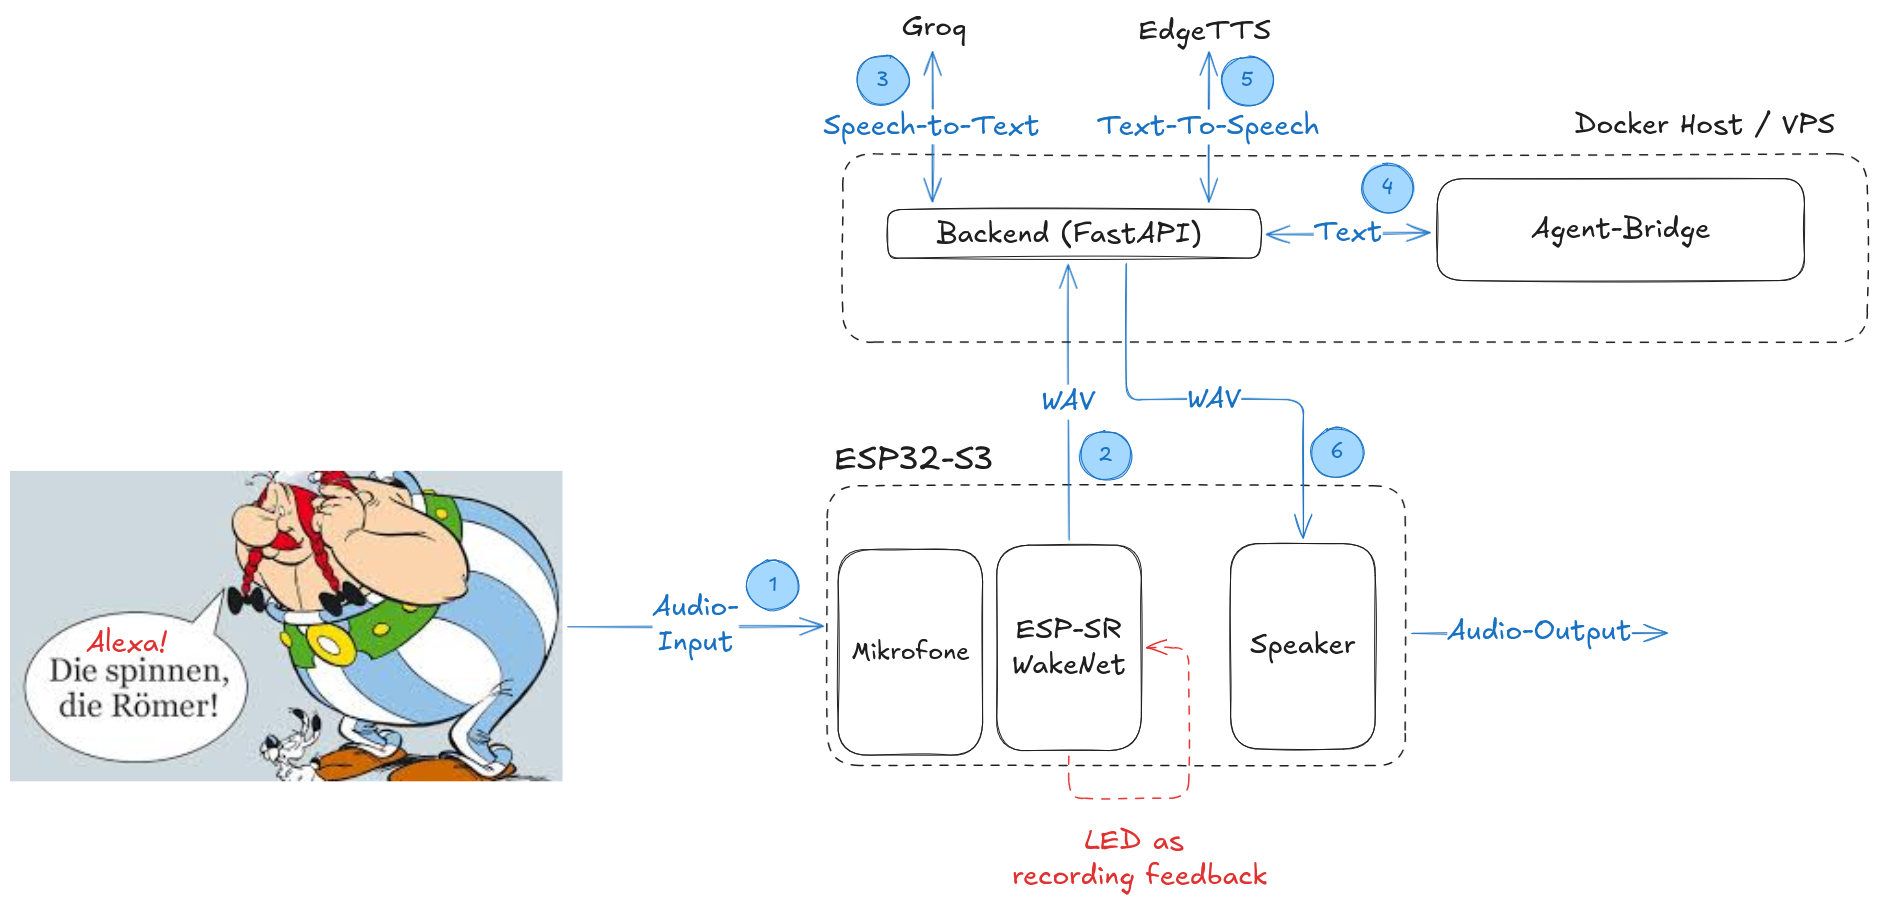
\includegraphics[width=0.8\textwidth]{graph.png}
    \caption{(1) Der ESP32-S3 verarbeitet den Audio-Input lokal mit ESP-SR WakeNet. Wenn das Wakeword erkannt wird (Alexa), startet die Aufnahme. Der LED-Ring des Audio-Boards leuchtet als Rückmeldung, dass gerade aufgenommen wird. Die Aufnahme enthält zusätzlich ca. 1,2 Sekunden Pre-roll, damit der Anfang der Frage nicht abgeschnitten wird. Danach läuft die Aufnahme weiter (bis 2,5 Sekunden Stille erkannt wird). (2) Diese WAV-Datei wird per HTTPS an das FastAPI-Backend (/chat/stream). (3) Das Backend schickt die WAV-Datei an die Groq API für Speech-to-Text. Aus dem Audio wird also Text. (4) Dieser Text geht vom FastAPI-Backend an die Agent Bridge. Die Agent-Bridge ist der TypeScript-Service, der die Pi-Agent-Session ausführt. Pi beantwortet dann die Nutzerfrage, zum Beispiel “Wie ist das Wetter heute?”. Die Textantwort kommt von der Agent Bridge zurück zum FastAPI-Backend. (5) Dort wird sie mit Edge TTS in Sprache umgewandelt. (6) Die WAV-Audio wird zurück an den ESP32 geschickt und abgespielt}
    \label{fig:graph}
\end{figure}


Die wichtigste Architekturentscheidung in diesem Prototyp ist die Trennung zwischen Agentenkern und Hardware-I/O. Mein Pi-driven Voice Agent läuft in einem separaten Docker-Host, während das ESP32-S3 Audio Board als austauschbarer Adapter für Mikrofon, Wakeword, Aufnahme, LED-Feedback und Wiedergabe dient.

Das Backend besteht aus der Backend API, der Agent Bridge und einem eigenen Pi-Profil. Dieses Profil enthält System Prompt, Settings, Extensions und Skills des Voice Agents. Die Struktur ist vom OpenClaw-Agent-Workspace-Gedanken inspiriert: Der Agent bekommt einen klaren eigenen Kontextbereich, in dem er arbeiten kann.


Während Wakeword und Audio-I/O gut auf den ESP32 passen, laufen STT- und TTS-Provider sowie der eigentliche Agentenworkflow über das Backend. So lassen sich Modelle, Provider und der eigentliche Agent ändern, ohne die Firmware des ESP32 neu bauen zu müssen. Mein Voice Agent in diesem Prototyp hat bewusst nur sehr eingeschränkte Tools bekommen: Er darf lokalen Kontext lesen und Websuche nutzen, aber keine Dateien schreiben und keine Shell ausführen. Eine Erweiterung über Read-only hinaus ist in Zukunft aber definitiv geplant.

Für Speech-to-Text nutze ich Groq mit \texttt{whisper-large-v3-turbo}, weil die Transkription durch spezialisierte Inferenz-Hardware sehr schnell ist und sich durch ein großzügiges kostenloses Tageskontingent kostengünstig nutzen lässt. Für Text-to-Speech verwende ich Edge TTS über die Python-Bibliothek \texttt{edge-tts}, weil es schnell reagiert und ohne zusätzliche TTS-Kosten brauchbare Sprachqualität liefert. OpenAI TTS wäre eine Alternative mit natürlicherem Klang, hätte aber Kosten- und Latenznachteile.

Grundsätzlich ist meine Architektur aber providerunabhängig gedacht. STT- und TTS-Provider lassen sich austauschen, und auch das LLM, das Pi intern verwendet, ist nicht fest vorgegeben. In meinen Tests nutze ich Pi über eine ChatGPT-Subscription (andere Providern wie Gemini, Kimi oder Claude wären natürlich auch möglich gewesen).



Hinweis: Der Rust CLI im Repo (backend/) ist ein zusätzlicher Testpfad. Er ersetzt nicht das ESP32-Board , macht aber den Backend- und Agentenfluss ohne Flashen und ohne Audio-Hardware prüfbar.

\section*{4. Umsetzung}

Nach dem Boot initialisiert der ESP32 Audio, LED, Wi-Fi, Backend-Verbindung und WakeNet. Danach wartet das Board lokal auf das Wakeword; erst dann startet Aufnahme und Backend-Kommunikation.

Nach erkanntem Wakeword startet die Session mit einem kurzen Pre-roll, damit der Anfang der Anfrage nicht abgeschnitten wird. Die Aufnahme endet nach einer erkannten 2,5s Stille und wird anschließend als WAV verpackt.

Die fertige WAV-Aufnahme wird per HTTPS an \texttt{/chat/stream} gesendet. Das Backend transkribiert die Aufnahme mit Groq, gibt den Text an die Agent Bridge weiter und erzeugt anschließend mit Edge TTS wieder Audio.

Provider-Zugangsdaten liegen bewusst im Backend. Der ESP32 kennt nur die Backend-URL und einen eigenen Token. Wenn Wi-Fi oder Backend nicht erreichbar sind, loggt der ESP32 den Fehler, gibt einen kurzen Error Beep als lokales Feedback an den Nutzer und gelangt wieder in den normalen Zustand (fällt also nicht aus).

Ergänzend zur obigen Beschreibung liegt im Repository-Root ein kurzes Demo-Video, welches den Ablauf praktisch zeigt: Wakeword, Aufnahme, Backendverarbeitung (inkl. Websuche, final/commentary-Antworten) und der eigentlichen Antwort über das Audio-Board.

\section*{6. Grenzen und Ausblick}

Der Voice-Agent ist nach wie vor prototypisch gehalten. Neben eingeschränktem Toolzugriff und Session-Control hat der Voice Agent eine recht hohen Latenz, da der ESP32 aktuell mit WAV arbeitet. Ein naheliegender nächster Schritt wäre komprimiertere Audioformate wie MP3 zu nutzen.

Auch das Wakeword ist zurzeit eine pragmatische Entscheidung. \texttt{Alexa} funktionierte in diesem Setup zuverlässig, während andere Modelle wie \texttt{Hey ESP} nicht stabil genug waren.

Ein weitere Lösung (für Latenzen und Wakeword) wäre es, stärkere Hardware, wie zum Beispiel ein Raspberry Pi, zu verwenden. So könnten Backend und Agent näher am Audio-Interface laufen und die Latenz stark gesenkt werden.

\end{document}
